\newpage
\section{Crystal Structure of Sodium Chloride (NaCl)}
\label{sec:NaCl}

\subsection*{Structural Analysis}

The following section, we are going to examine the structure of NaCl, the plot shows the obtained intensity distribution.

\begin{figure}[h]
    \centering
    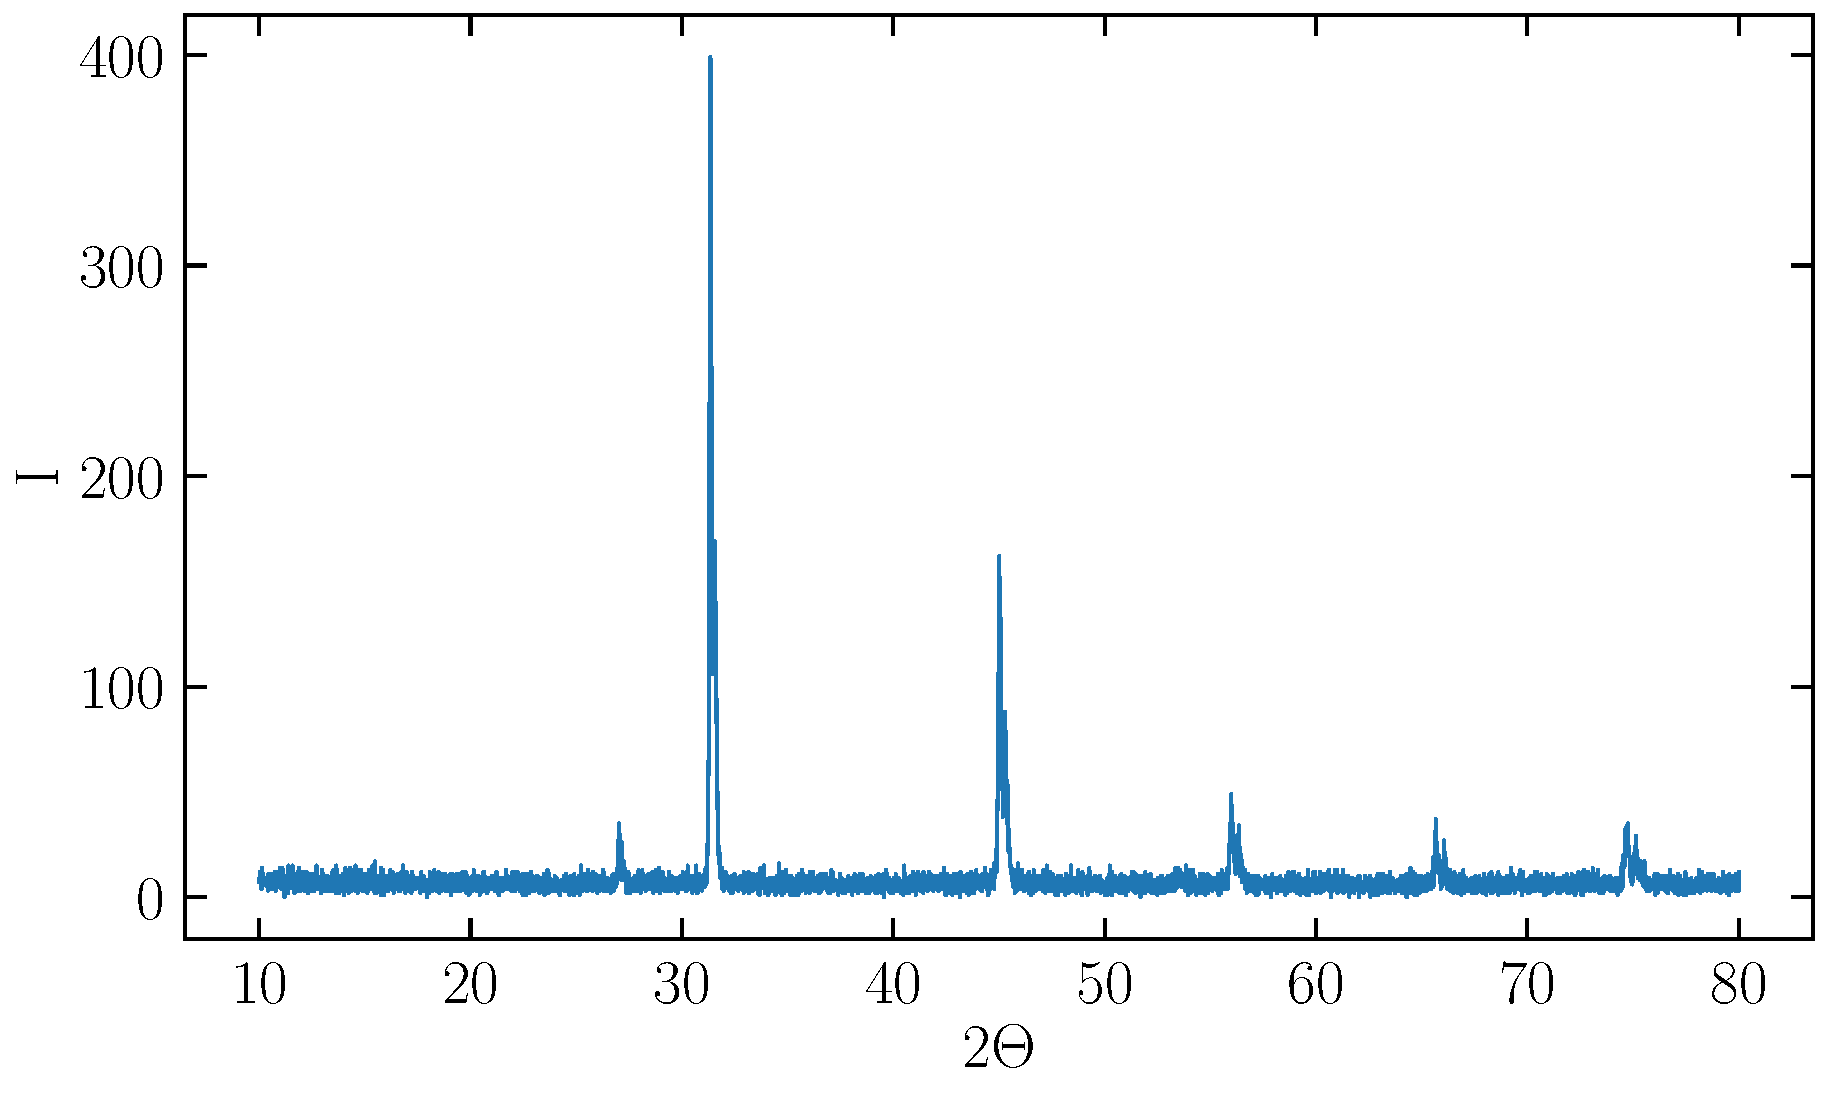
\includegraphics[width=\textwidth]{Pictures/Evaluation/42/IntDistNaCl.pdf}
    \caption{Intensity distribution of the NaCl experiment.}
\end{figure}

The following table shows the intensity, the full width at half maximum (FWHM) and the positions of each peak.

\begin{table}[ht]
    \centering
    \begin{tabular}{c|c c c}
        \hline
        Peak No. &  2$\theta_{fit}$ / \SIUnitSymbolDegree &  $I_{fit}$ / a.u. &   $FWHM$ / \SIUnitSymbolDegree \\
        \hline
            1 &    27.15 &   0.05 &  0.11 \\
            2 &    31.48 &   0.86 &  0.12 \\
            3 &    45.02 &   0.48 &  0.16 \\
            4 &    53.62 &   0.03 &  0.18 \\
            5 &    56.21 &   0.15 &  0.19 \\
            6 &    65.66 &   0.10 &  0.22 \\
            7 &    72.70 &   0.02 &  0.24 \\
            8 &    74.70 &   0.17 &  0.25 \\
        \hline
    \end{tabular}
    \caption{Fit values for each peak in the intensity distribution.}
    \label{tab:fitVals}
\end{table}

Using the following realtions:

Bragg condition: 
\begin{align}
    2d sin(\Theta) = m \lambda
\end{align}

Distance between to planes in a cubic system:
\begin{align}
    d = \frac{a^2}{h^2+k^2+l^2}
\end{align}
with the laue indices $h, h, l$ and the lattice parameter $a$.

In the following we assume $m=1$.
So we can derive the following equation:
\begin{align}
    sin^2(\Theta) = (h^2+k^2+l^2)\frac{\lambda^2}{4a^2}
\end{align}
We define the constant: $c^{-1} = \frac{\lambda^2}{4a^2}$, which depends only on the setup.

We can write an equation to compute $a$:
\begin{align}
    a=\sqrt{c}\frac{\lambda}{2}
\end{align}

Using this relations and the date from table \ref{tab:fitVals} we get the values displayed in the following table (table \ref{tab:latticeParams}):

\begin{table}[h]
    \centering
    \begin{tabular}{c | c c c c c c c}
        \hline
        Peak No. &  2$\theta_{fit}$ / \SIUnitSymbolDegree &    $d$ / \SIUnitSymbolAngstrom &  $\sin^2(\theta)$ &  $\frac{\lambda^2}{4a^2}$ &  $h^2+k^2+l^2$ &    $a$ / \SIUnitSymbolAngstrom &   (h k l) \\
        \hline
        1 &   27.15 & 3.28 & 0.055 &     0.018 &       3 & 5.682 & (1 1 1) \\
        2 &   31.48 & 2.84 & 0.074 &     0.018 &       4 & 5.677 & (0 0 2) \\
        3 &   45.02 & 2.01 & 0.147 &     0.018 &       8 & 5.689 & (2 0 2) \\
        4 &   53.62 & 1.71 & 0.203 &     0.018 &      11 & 5.662 & (1 1 3) \\
        5 &   56.21 & 1.63 & 0.222 &     0.018 &      12 & 5.662 & (2 2 2) \\
        6 &   65.66 & 1.42 & 0.294 &     0.018 &      16 & 5.681 & (0 0 4) \\
        7 &   72.70 & 1.30 & 0.351 &     0.018 &      19 & 5.663 & (3 1 3) \\
        8 &   74.70 & 1.27 & 0.368 &     0.018 &      20 & 5.676 & (2 0 4) \\
        \hline
    \end{tabular}
    \caption{Lattice parameters and indices for each peak fitted.}
    \label{tab:latticeParams}
 \end{table}

 On average, the lattice parameter is $ a = 5.674$. This fizs pretty well with the literature value os $a=5.64$ (Wikipedia).